\subsection{Modeling Language for System Design}
\label{sec:modelingLanugage}
Figure~\ref{fig:proposed_safety_process} presents our proposed use of a single unified model to support both system design and safety analysis. It describes both system design and safety-relevant information 
that are kept distinguishable and yet are able to interact with each other. The shared model is a living model that captures the current state of the system design as it moves through the development lifecycle, allowing all participants of the ARP4754A process to be able to communicate and review the system design. Safety analysis artifacts can be generated directly from the model, 
providing
the capability to more accurately analyze complex systems.

\begin{figure}[t!]
	
	\centering
	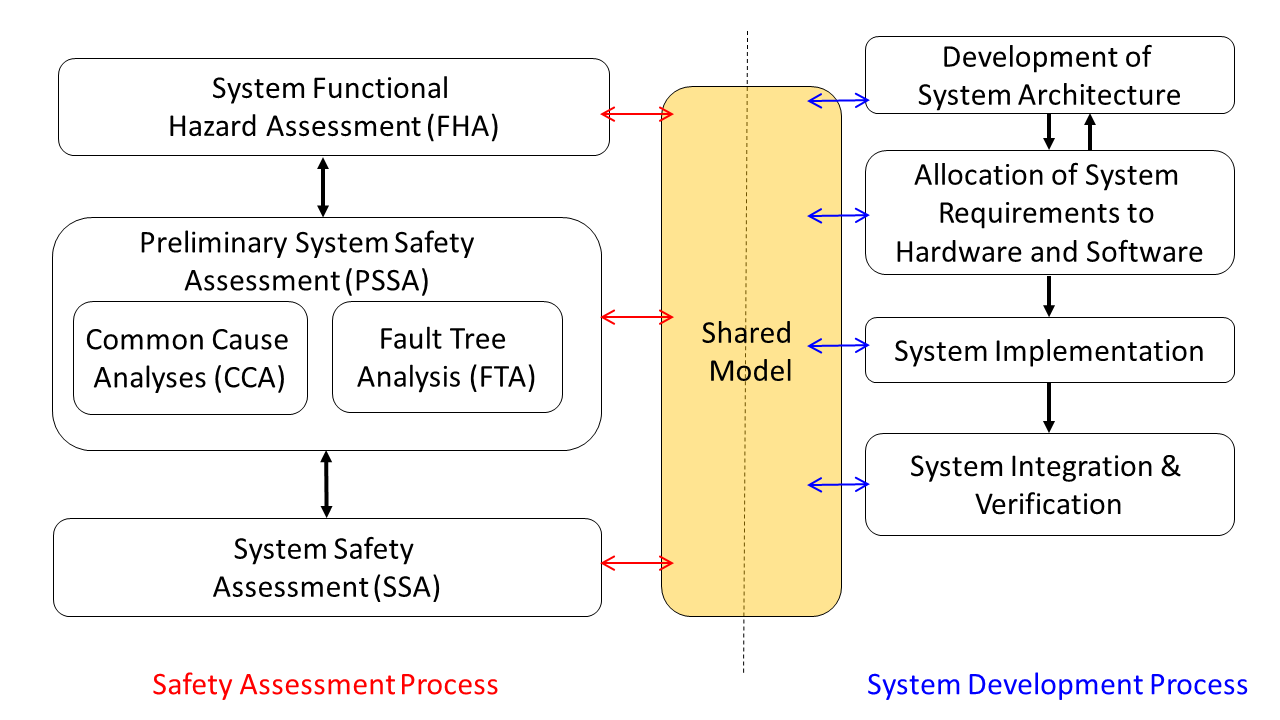
\includegraphics[trim=0 5 0 5,clip,width=0.85\textwidth]{images/process3.png}
	
	\caption{Use of the Shared System/Safety Model in the ARP4754A Safety Assessment Process}
	\label{fig:proposed_safety_process}
\end{figure}

The Architectural Analysis and Design Language (AADL)~\cite{FeilerModelBasedEngineering2012} to construct system architecture models.  AADL is an SAE International standard that defines a language and provides a unifying framework for describing the system architecture for ``performance-critical, embedded, real-time systems''~\cite{AADL_Standard}. From its conception, AADL has been designed for the design and construction of avionics systems.  
Rather than being merely descriptive, AADL models can be made specific enough to support system-level code generation.  Thus, results from analyses conducted, including the new safety analysis proposed here, correspond to the system that will be built from the model.  

An AADL model describes a system in terms of a hierarchy of components and their interconnections, where each component can either represent a logical entity (e.g., application software functions, data) or a physical entity (e.g., buses, processors). An AADL model can be extended with language annexes to provide a richer set of modeling elements for various system design and analysis needs (e.g., performance-related characteristics, configuration settings, dynamic behaviors). The language definition is sufficiently rigorous to support formal analysis tools that allow for early phase error/fault detection.

The Assume Guarantee Reasoning Environment (AGREE)~\cite{NFM2012:CoGaMiWhLaLu} is a tool for formal analysis of behaviors in AADL models.  AGREE is implemented as an AADL annex and annotates AADL components with formal behavioral contracts. Each component's contracts can include assumptions and guarantees about the component's inputs and outputs respectively, as well as predicates describing how the state of the component evolves over time. AGREE translates an AADL model and the behavioral contracts into Lustre~\cite{Halbwachs91:IEEE} and then queries a user-selected
model checker to conduct the back-end analysis. The analysis %is
can be performed compositionally following the architecture hierarchy such that analysis at a higher level is based on the components at the next lower level.  When compared to monolithic analysis (i.e., analysis of the flattened model composed of all components), the compositional approach allows the analysis to scale to much larger systems~\cite{NFM2012:CoGaMiWhLaLu}. 

%In the avionics context, the software functions/applications, the hardware equipment, and the system that is composed of their integration can all be represented as components connected to/composed of/bind to other components in a hierarchical AADL model. AGREE contracts can be used to capture the functional requirements at each level of the hierarchy. Once the model has been reviewed and the requirements captured have been validated, the back-end analysis can be conducted to verify if each level of the model implements its higher level requirements correctly.

%AADL with the AGREE extension serves as a good candidate as the modeling language for describing the system design aspects of a shared system design and safety analysis model. 
In our prior work~\cite{Stewart17:IMBSA}, we added an initial failure effect modeling capability to the AADL/AGREE language and tool set.  We are continuing this work so that our tools and methodology can be used to satisfy system safety objectives of ARP4754A and ARP4761.  

\begin{comment}
In particular, our goals are to:

\begin{itemize}
	\item Provide a comprehensive, qualitative description of the causal relationship between basic failure events and system level safety requirements.
	\item Provide an accurate, quantitative description of the contribution relationship between failure rates of the fault tree basic events and numerical probability requirements at the system level.
\end{itemize}
\end{comment}
%The remainder of the paper describes our approach towards both of the goals.





\subsubsection{Faults, Errors, and Failures}
\label{sec:terminology}
\danielle{Note sure where this should go for now.}
The usage of the terms error, failure, and fault are defined in ARP4754A~\cite{SAE:ARP4754A} and are described here for ease of understanding. A \textit{failure} is an event that occurs when the delivered service of a system deviates from correct behavior. A service of a system is a sequence of the system's external states. This means that if a service failure occurs, one or more of the systems external states has deviated from the correct service state. This deviation is called an \textit{error}. The complete definition of an error is the part of the state of the system that may cause a failure. Not all errors will affect the external state of a system and cause an failure. The cause of an error is a \textit{fault}. Faults can be \textit{active} or \textit{dormant}. A fault is active when it causes an error to occur, else it is dormant.

\iffalse
\begin{figure*}
	%\vspace{-0.956in}
	\centering
	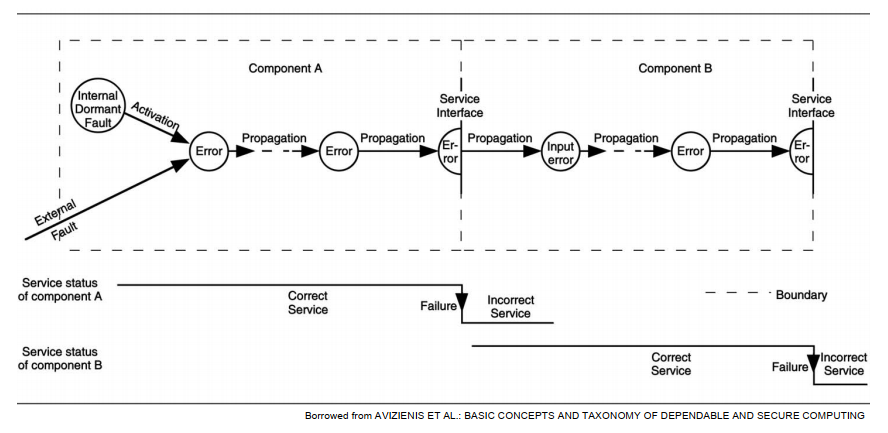
\includegraphics[width=1.0\textwidth]{images/fault_error_failure.png}
	%\vspace{-0.4in}
	\caption{Faults, Errors, and Failures}
	\label{fig:fault_error_failure}
\end{figure*}
\fi

The relationship between faults, failures, and errors were summarized by Aviyienis, et. al.~\cite{basicConcepts} and are described here once again.% and is shown in Figure~\ref{fig:fault_error_failure}.

\begin{itemize}
\item A fault is active when it causes an error. An active fault can be an internal fault that was previously dormant but has been activated or it can be an external fault. Fault activation is what causes a dormant fault to become active. 

\item Error propagation in a component is caused by the computation process of that component. In this process, an error is successfully transformed into other errors. Error propagation from component A to component B occurs when an error reaches the service interface of component A. The service delivered from component A to component B is no longer correct and thus the error is propagated into component B through the interface between the two components.

\item A service failure occurs when that error is propagated to the service interface and causes the service of the system to be incorrect. The failure of a component causes a fault in the system that contains the component. Service failure of a system will cause external fault(s) for the other systems that recieve service from the given system. 
\end{itemize}